\documentclass[a4paper,11pt]{article}
\usepackage[margin=2cm]{geometry}

\usepackage[nodayofweek]{datetime}
\usepackage{cite}
\usepackage{graphicx}
\longdate

\usepackage{hyperref}
\usepackage{fancyhdr}
\pagestyle{fancyplain}
\fancyhf{}
\lhead{\fancyplain{}{M.Sc.\ Group Project Report}}
\rhead{\fancyplain{}{\today}}
\cfoot{\fancyplain{}{\thepage}}


\title{Implementation of attentional bistability of the dragonfly visual neurons in an intelligent biomimetic agent\\\Large{--- Final Report ---}}
\author{Juan Carlos Farah, Panagiotis Almpouras, Ioannis Kasidakis, Erik Grabljevec, Christos Kaplanis\\
       \{jcf214, pa512, ik311, eg1114, ck2714\}@doc.ic.ac.uk\\ \\
       \small{Supervisors: Professor Murray Shanahan, Zafeirios Fountas, Pedro Mediano}\\
       \small{Course: CO530/533, Imperial College London}
}

\begin{document}
\maketitle

\section{Design}

The challenge of designing a tool that could satisfy the overall functionality outlined in the introduction could be distilled down to two main facets:
\begin{enumerate}
\item Deciding on the components of the dragonfly visual system and how they would be connected together.
\item Deciding on the user interface and specifying an API for the system.
\end{enumerate}

\subsection{Components}

Having consulted academic research on the subject of dragonfly vision and discussed with our supervisors, we managed to identify five key components we would need to model in order to implement a coherent system. 

\begin{enumerate}
\item{Target Animation:} An animated video that provides the visual input to the system, emulating the retina of the dragonfly. User should be able to specify movements of multiple targets within the visual field and choose the background.
\item{Elementary Small Target Motion Detector (ESTMD):} The ESTMD neurons are the first layer of visual processing in the dragonfly. They have the general function of identifying and isolating small moving targets, even against a cluttered, moving background (WIEDERMAN 2008). They take arrays of pixel values as input from the animation and output firing rates of neurons to be processed by the next layer.
\item{Centrifugal Small Target Motion Detector (CSTMD):} The CSTMD neuron is a higher order visual neuron in the brain of the dragonfly. This neuron reacts to the presentation of multiple visual stimuli by firing as if only one of the stimuli was present \cite{w13}. The CSTMD takes the firing rates of the ESTMD as input and outputs a time series of neuron spikes (spike trains) to the next layer.
\item{Pattern Recognition:} This module has the function of detecting patterns in the output of the CSTMD in order to distil features of target movement within the visual field. While it does not have an exact correspondence to a layer of neurons in the dragonfly, it uses a well-established biological learning mechanism called Spike Timing Dependent Plasticity (STDP) \cite{stdp1}\cite{stdp2}. It outputs spike trains to the Action Selection module.
\item{Action Selection:} Using reward-modulated reinforcement learning along with the output of the pattern recognition neurons this module is responsible for the movement of the dragonfly towards the animated target.It includes an animation component for the visualisation of the outcome.
\end{enumerate}

\subsection{User Interface}
Although this is not a module that is actively implicated in the neural processes that are being modelled in this project, it is a very powerful tool that drastically enhances the functionality of the system. The web client is connected to every component providing a user friendly interface that allows not only the independent use of each of the components but also to run simulations using the system as a whole. The web client provides the user with an output that is crucial in understanding the performance of the system. It allows for flexibility as the users may set their own parameters and run, save and load simulations. Similarly to the target animation there were many options in terms of the software development tools we could use for for the implementation of the web client. Python was chose to allow for a uniform design throughout the project.


The following figure provides a graphical representation of the system as whole. The animated target acts as input to the ESTMD neuron which identifies and isolates the small targets (if any) by processing each frame of the animation. The output of the ESTMD is yet another animation but this time the only things visible are the small targets. This new animation acts as input to the CSTMD neuron. In the presence of multiple targets, a well behaved CSTMD neuron should select one and translate only that target's movement into a spike train which will be processed by the pattern recognition neurons. In this spike train a pattern exists that encodes information about the direction of the selected target. The pattern recognition neuron trained to identify that particular pattern will fire - upon recognition of the pattern - while inhibiting the rest of the pattern recognition neurons. The action selection mechanism then has to translate the output of the pattern recognition (i.e. the spike from a neuron) to an action that ideally will bring the dragonfly closer to its prey.
The web client "oversees" the whole process ensuring that the components are well connected and provides the user with key metrics regarding the performance of the system (or an individual module) for a particular simulation. The database stores animations, simulations and their respective results enabling their reloading if a future reference is desired.

\begin{figure}[hb]
\centering
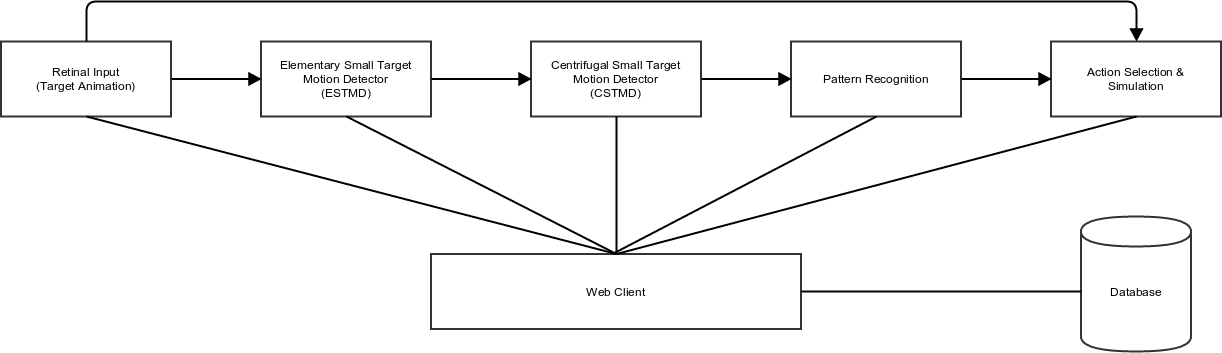
\includegraphics[scale = 0.35]{designblockdiagram2}
\caption{Project Structure Diagram.}
\end{figure}


The programming language used throughout the project was Python \cite{python}. Python includes libraries that allow for efficient matrix manipulations that were key in most of the modules. Matlab was an alternative we initially considered \cite{matlab}. Although Matlab is very powerful and user friendly for some particular tasks, it does not allow for the flexibility that Python does. For that reason Matlab was disregarded as an option.
The database we used was MongoDB because of the increasing popularity of the distributed databases as well as the fact that this was the database scheme we were most familiar with.




\end{document}

